\documentclass[a4paper]{article}

\usepackage[francais]{babel}
\usepackage[utf8]{inputenc}
\usepackage[OT1]{fontenc}
\usepackage{amsmath}
\usepackage{amssymb}
\usepackage{graphicx}
\usepackage{url}
\usepackage{subfigure}

\usepackage[]{fullpage}

\graphicspath{ {./imgs/} }

\title{Configuration et sécurisation de services réseaux}
\author{Sophie VALENTIN, Mathieu BIVERT}

\makeatletter
\def\thickhrulefill{\leavevmode \leaders \hrule height 1pt\hfill \kern \z@}
\def\maketitle{
	\null
	\thispagestyle{empty}
	\vskip 1cm
	\begin{center}
		\normalfont\large\huge\@author
	\end{center}
	\vfil
	\vfil
	\vfil
	\vfil
	\vfil
	\vfil
	\vfil
	\vfil
	\vfil
	\vfil
	\vfil
	\hrule height 2pt
	\par
	\begin{center}
				\huge \strut \@title \par
				\@date
	\end{center}
	\hrule height 2pt
	\par
	\vfil
	\vfil
	\vfil
	\vfil
	\vfil
	\vfil
	\vfil
	\vfil
	\vfil
	\vfil
	\vfil
	\vfil
	\vfil
	\vfil
	\vfil
	\vfil
	\vfil
	\vfil
	\vfil
	\vfil
	\vfil
	\vfil
	\vfil
	\vfil
	\vfil
	\begin{center}
  			\huge Professeur : Bruno MARTIN
    \end{center}
	\null
	\begin{figure}[!ht]
		\centering
		
\includegraphics[scale=.5]{polytech.png}
	\end{figure}
	\vfil
	\cleardoublepage
}
\makeatother

\begin{document}
\maketitle

\newpage
\tableofcontents

\newpage

\section{Topologie}
\section{Mise en place d'une passerelle réseau}
\subsection{Configuration de la passerelle}
Configuration de l'interface en mode NAT (bridged aurait été
un choix valide aussi).
\begin{verbatim}
(passerelle)# dhclient em0
DHCPREQUEST on em0 to 255.255.255.255 port 67
DHCPACK from 192.168.237.254
bound to 192.168.237.132 -- renewal in 900 seconds.
\end{verbatim}

Normalement déjà activé au démarrage:
\begin{verbatim}
(passerelle)# grep em0 /etc/rc.conf 
ifconfig_em0="DHCP"
\end{verbatim}

Puis l'interface connectée à un réseau local:
\begin{verbatim}
(passerelle)# ifconfig em1 192.168.98.2
\end{verbatim}

Au démarrage:
\begin{verbatim}
(passerelle)# cat >> /etc/rc.conf
ifconfig_em1="inet 192.168.98.2 netmask 255.255.255.0"
^D
\end{verbatim}

On s'assure que l'on peut bien communiquer avec le système hôte
via les deux interfaces, et que l'on peut accéder aux Internets:
\begin{verbatim}
(passerelle)# for i in 192.168.98.1 192.168.237.1 google.fr; do ping -c1 -q $i; done
PING 192.168.98.1 (192.168.98.1): 56 data bytes

--- 192.168.98.1 ping statistics ---
1 packets transmitted, 1 packets received, 0.0% packet loss
round-trip min/avg/max/stddev = 0.217/0.217/0.217/0.000 ms
PING 192.168.237.1 (192.168.237.1): 56 data bytes

--- 192.168.237.1 ping statistics ---
1 packets transmitted, 1 packets received, 0.0% packet loss
round-trip min/avg/max/stddev = 0.117/0.117/0.117/0.000 ms
PING google.fr (173.194.34.24): 56 data bytes

--- google.fr ping statistics ---
1 packets transmitted, 1 packets received, 0.0% packet loss
round-trip min/avg/max/stddev = 50.611/50.611/50.611/0.000 ms
\end{verbatim}

Activation IP forwarding:
\begin{verbatim}
(passerelle)# sysctl net.inet.ip.forwarding=1
net.inet.ip.forwarding: 0 -> 1
\end{verbatim}

% http://docs.freebsd.org/doc/4.6.2-RELEASE/usr/share/doc/en_US.ISO8859-1/books/ppp-primer/x237.html
Pour l'avoir au démarrage:
\begin{verbatim}
(passerelle)# cat >> /etc/rc.conf
gateway_enable="YES"
^D
\end{verbatim}

% http://freebsd.rogness.net/redirect.cgi?basic/nat.html
Par défault, le noyau de FreeBSD n'est pas configuré pour
faire du NAT; il recompiler un pépin en lui ajoutant la
bonne option:
\begin{verbatim}
(passerelle)# cd /sys/i386/conf/
(passerelle)# cp GENERIC LOCAL
(passerelle)# cat >> LOCAL
options         IPDIVERT                # Divert packets
^D
(passerelle)# config LOCAL
Kernel build directory is ../compile/LOCAL
Don't forget to do ``make cleandepend && make depend''
(passerelle)# cd ../compile/LOCAL/ && make cleandepend && make depend && make && make install
…
kldxref /boot/kernel
\end{verbatim}

% http://www.freebsd.org/doc/en_US.ISO8859-1/books/handbook/network-natd.html
Avant de redémarrer sur le nouveau noyau, on s'assure
\begin{enumerate}
	\item le firewall \& natd soient activés au démarrage;
	\item un script personnalisé défini les règles du firewall;
	\item les options noyaux pour le NAT soient préchargés par le bootloader;
	\item le firewall soit le plus laxiste possible dans un premier temps.
\end{enumerate}
\begin{verbatim}
(passerelle)# cat >> /etc/rc.conf
firewall_enable="YES"
firewall_type="OPEN"
firewall_script="/etc/fw.sh"
natd_enable="YES"
# interface de sortie
natd_interface="em0"
^D
(passerelle)# cat >> /boot/loader.conf
ipfw_load="YES"
ipdivert_load="YES"
net.inet.ip.fw.default_to_accept="1"
^D
(passerelle)# reboot
\end{verbatim}

Par défault, syslogd est activé:
\begin{verbatim}
(passerelle)# ps aux| grep sysl
root  1140  0.0  0.6  9504 1504 ??  Ss    3:54AM  0:00.02 /usr/sbin/syslogd -s
root  1419  0.0  0.7  9636 1688  0  S+    4:20AM  0:00.00 grep sysl
(passerelle)# tail -5 /var/log/auth.log
Feb  6 03:50:41 passerelle su: cssr to root on /dev/pts/0
Feb  6 03:54:06 passerelle sshd[1237]: Server listening on :: port 22.
Feb  6 03:54:06 passerelle sshd[1237]: Server listening on 0.0.0.0 port 22.
Feb  6 03:54:29 passerelle sshd[1307]: Accepted keyboard-interactive/pam for cssr from 192.168.237.1 port 42087 ssh2
Feb  6 03:54:31 passerelle su: cssr to root on /dev/pts/0
\end{verbatim}

\subsection{Configuration du client}
Configuration de l'\og interface \fg\ réseau, ajout d'une route par
défaut, et contact de la machine hôte via la passerelle:
\begin{figure}[!ht]
	\centering
	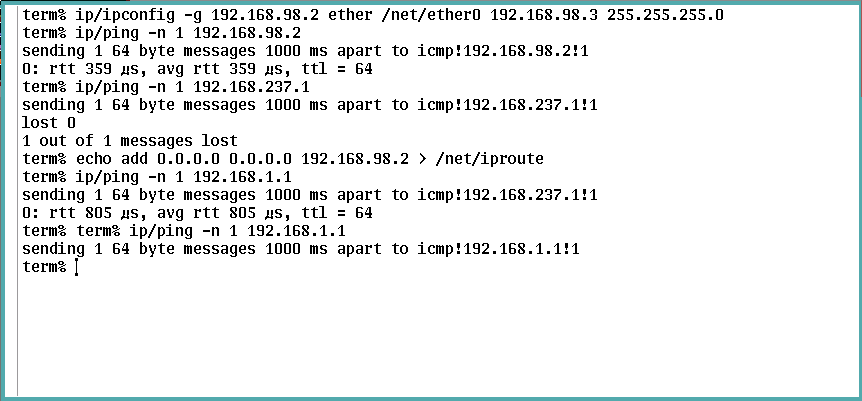
\includegraphics[scale=.5]{ipconfig.png}
\end{figure}

\subsection{Mise en place d'accès distants sur la passerelle}
\subsubsection{Telnet}
Activation via inetd:
\begin{verbatim}
(passerelle)# ed /etc/inetd.conf 
5014
/tel
#telnet stream  tcp     nowait  root    /usr/libexec/telnetd    telnetd
s/^#/
telnet  stream  tcp     nowait  root    /usr/libexec/telnetd    telnetd
wq
5013
(passerelle)# cat >> /etc/rc.conf 
inetd_enable="YES"
^D
(passerelle)# /etc/rc.d/inetd start
Starting inetd.
(passerelle)# echo 'Welcome!' > /etc/motd
\end{verbatim}

On essaye de se connecter depuis le client:
\begin{figure}[!ht]
	\centering
	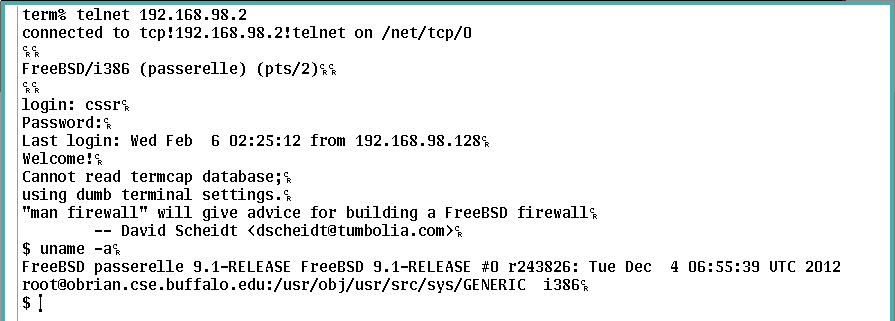
\includegraphics[scale=.5]{telnet.png}
\end{figure}

Comme les paquets passent par des interfaces virtuelles, on
peut les observer depuis la machine hôte sans avoir à se
mettre en homme du milieu. On se reconnecte avec wireshark
démarré sur l'hôte:
\begin{figure}[!ht]
	\centering
	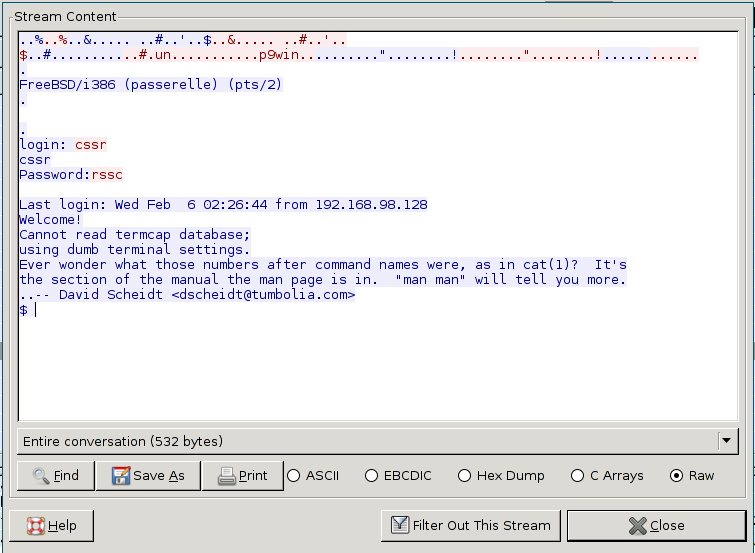
\includegraphics[scale=.5]{telnetsniff.png}
\end{figure}

\subsubsection{SSH}
Normalement activé au démarrage
\begin{verbatim}
(passerelle)# grep ssh /etc/rc.conf 
sshd_enable="YES"
\end{verbatim}

% http://plan9.bell-labs.com/wiki/plan9/ssh_configuration/
Le client ssh plan9 ne fonctionne qu'avec la version $1$ du
protocole (une version incomplète de la version $2$ est
disponibles dans \textit{/n/contrib/blstuart/ssh}). On modifie
donc la version du protocole, et on redémarre le service:
\begin{verbatim}
(passerelle)# grep Protocol /etc/ssh/sshd_config
Protocol 1
(passerelle)# /etc/rc.d/sshd restart
Stopping sshd.
Starting sshd.
\end{verbatim}

Côté client, on génère une clef RSA que l'on convertie ensuite
au format requis pour ssh, puis on copie cette version sur la
passerelle, et enfin, on donne la clef au gestionnaire de clefs du
client (factotum):
\begin{figure}[!ht]
	\centering
	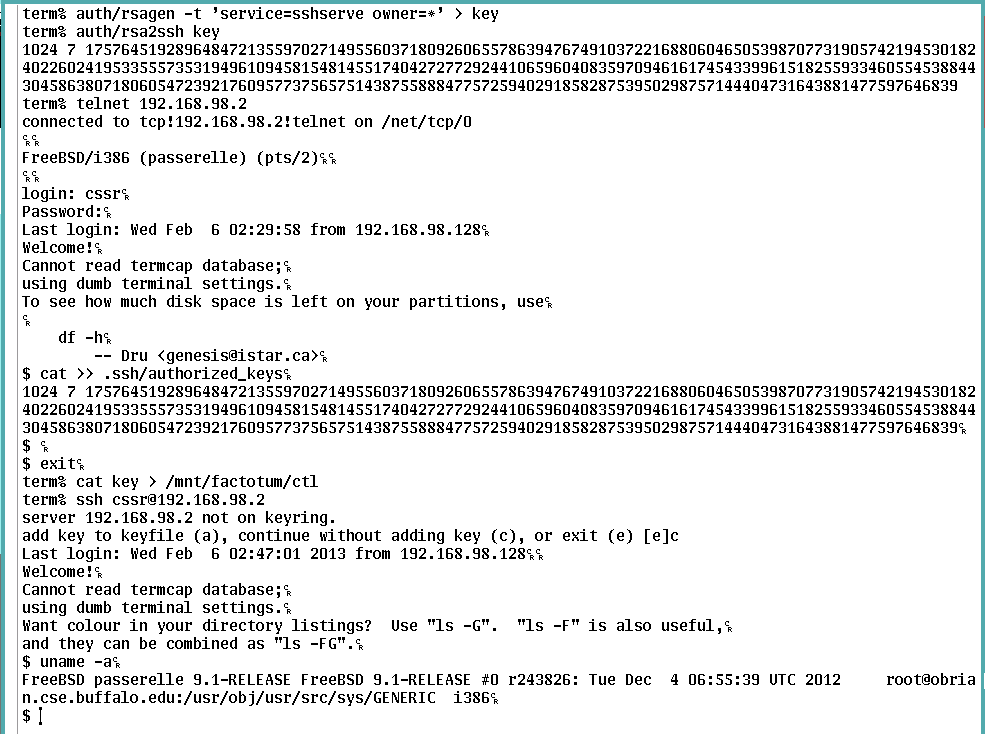
\includegraphics[scale=.5]{sshv1.png}
\end{figure}

\subsection{Nmap}
Depuis le système hôte:
\begin{verbatim}
(redox)# nmap -A 192.168.98.2

Starting Nmap 6.25 ( http://nmap.org ) at 2013-02-06 04:24 CET
Nmap scan report for 192.168.98.2
Host is up (0.0011s latency).
Not shown: 998 closed ports
PORT   STATE SERVICE VERSION
22/tcp open  ssh     OpenSSH 5.8p2_hpn13v11 (FreeBSD 20110503; protocol 2.0)
| ssh-hostkey: 1024 ad:53:43:8e:1e:9a:25:59:ef:d7:16:99:d1:21:47:a0 (DSA)
| 2048 ab:d7:19:4c:99:73:6e:f3:0b:ba:56:95:1e:67:92:6d (RSA)
|_256 8a:e1:0c:ab:21:3e:14:4b:74:f4:95:0d:02:f0:21:d3 (ECDSA)
23/tcp open  telnet  BSD-derived telnetd
MAC Address: 00:0C:29:A7:72:B4 (VMware)
Device type: general purpose
Running: FreeBSD 7.X|8.X|9.X|10.X
OS CPE: cpe:/o:freebsd:freebsd:7 cpe:/o:freebsd:freebsd:8 cpe:/o:freebsd:freebsd:9 cpe:/o:freebsd:freebsd:10
OS details: FreeBSD 7.0-RELEASE-p1 - 10.0-CURRENT
Network Distance: 1 hop
Service Info: OS: FreeBSD; CPE: cpe:/o:freebsd:freebsd

TRACEROUTE
HOP RTT     ADDRESS
1   1.10 ms 192.168.98.2

OS and Service detection performed. Please report any incorrect results at http://nmap.org/submit/ .
Nmap done: 1 IP address (1 host up) scanned in 9.31 seconds
\end{verbatim}

\section{Mise en place d'un serveur HTTP, et HTTPS}
\subsection{Installation des logiciels}
\subsubsection{OpenSSL}
Déjà installé, avec la version qui-va-bien:
\begin{verbatim}
(passerelle)# openssl version
OpenSSL 0.9.8x 10 May 2012
\end{verbatim}
\subsubsection{Apache2}
D'après la documentation, pas besoin d'installer depuis les ports
pour avoir un support d'SSL:
\begin{verbatim}
(passerelle)# PACKAGESITE=ftp://ftp.freebsd.org/pub/FreeBSD/ports/i386/packages/Latest/ pkg_add -r apache22
…
(passerelle)# cat >> /etc/rc.conf
apache22_enable="YES"
^D
\end{verbatim}

On s'assure que le système est capable de se connaître via son hostname,
et on démarre apache:
\begin{verbatim}
(passerelle)# ping passerelle
ping: cannot resolve passerelle: Unknown host
(passerelle)# grep ^127.0.0.1 /etc/hosts
127.0.0.1               localhost localhost.my.domain
…
(passerelle)# grep ^127.0.0.1 /etc/hosts
127.0.0.1               localhost localhost.my.domain passerelle
passerelle)# ping -q -c 1 passerelle
PING localhost (127.0.0.1): 56 data bytes

--- localhost ping statistics ---
1 packets transmitted, 1 packets received, 0.0% packet loss
round-trip min/avg/max/stddev = 0.031/0.031/0.031/0.000 ms
(passerelle)# grep ^ServerName /usr/local/etc/apache22/httpd.conf 
ServerName passerelle:80
(passerelle)# service apache22 start
Performing sanity check on apache22 configuration:
Syntax OK
Starting apache22.
(passerelle)# nc passerelle 80
GET /
<html><body><h1>It works!</h1></body></html>(passerelle)# 
\end{verbatim}

\subsection{Passage à HTTPS}
\subsubsection{Création d'un certificat auto-signé}
Le même certificat sera aussi utilisé pour dovecot, postfix, etc.

Création de la clef privée:
\begin{verbatim}
(passerelle)# openssl genrsa -out ca.key 1024
Generating RSA private key, 1024 bit long modulus
.......++++++
.....................................................++++++
e is 65537 (0x10001)
\end{verbatim}

Création du CSR (Certificate Signing Request):
\begin{verbatim}
(passerelle)# openssl req -new -key ca.key -out ca.csr
You are about to be asked to enter information that will be incorporated
into your certificate request.
What you are about to enter is what is called a Distinguished Name or a DN.
There are quite a few fields but you can leave some blank
For some fields there will be a default value,
If you enter '.', the field will be left blank.
-----
Country Name (2 letter code) [AU]:FR
State or Province Name (full name) [Some-State]:France
Locality Name (eg, city) []:Nice
Organization Name (eg, company) [Internet Widgits Pty Ltd]:CSSR Ltd
Organizational Unit Name (eg, section) []:
Common Name (e.g. server FQDN or YOUR name) []:
Email Address []:

Please enter the following 'extra' attributes
to be sent with your certificate request
A challenge password []:A challenge password
An optional company name []:
\end{verbatim}

Création du certificat X$509$:
\begin{verbatim}
(passerelle)# openssl x509 -req -days 365 -in ca.csr -signkey ca.key -out ca.crt
Signature ok
subject=/C=FR/ST=France/L=Nice/O=CSSR Ltd
Getting Private key
\end{verbatim}

Et on copie dans un répértoire adéquat:
\begin{verbatim}
(passerelle)# cp ca.* /etc/ssl/
\end{verbatim}

\subsubsection{Configuration d'apache}

\begin{verbatim}
(passerelle)# ed httpd.conf 
16777
/httpd-ssl.conf
#Include etc/apache22/extra/httpd-ssl.conf
s/^#/
Include etc/apache22/extra/httpd-ssl.conf
wq
16776
\end{verbatim}

Modification liens vers clefs/certificats
\begin{verbatim}
(passerelle)# ed extra/httpd-ssl.conf
11002
/^SSLCe
SSLCertificateFile "/usr/local/etc/apache22/server.crt"
s, ".*, "/etc/ssl/ca.crt"
SSLCertificateFile "/etc/ssl/ca.crt"
/^KeyFi
?
/KeyFi
SSLCertificateKeyFile "/usr/local/etc/apache22/server.key"
s, ".*, "/etc/ssl/ca.key"
SSLCertificateKeyFile "/etc/ssl/ca.key"
wq
10960
\end{verbatim}

Modification chemin vers fichiers:
\begin{verbatim}
#   General setup for the virtual host
DocumentRoot "/export/wwws/"
ServerName www.example.com:443
ServerAdmin you@example.com
ErrorLog "/var/log/httpd-error.log"
TransferLog "/var/log/httpd-access.log"

<Directory /export/wwws>
        Options FollowSymLinks
        AllowOverride None
        Order deny,allow
</Directory>
\end{verbatim}

On redémarre:
\begin{verbatim}
(passerelle)# mkdir -p /export/wwws/
(passerelle)# echo '<html><p>hello, world</p></html>' > /export/wwws/index.html
(passerelle)# service apache22 restart
Performing sanity check on apache22 configuration:
Syntax OK
Stopping apache22.
Waiting for PIDS: 2565.
Performing sanity check on apache22 configuration:
Syntax OK
Starting apache22.
\end{verbatim}
samarsh (tm)

TODO ajouter httpd dans inetd

\subsection{Page d'authentification (page de création de compte?)}
\subsection{Firewall le retour}

\section{Comptes emails}
TOCLEAN
\begin{verbatim}
(passerelle)# PACKAGESITE=ftp://ftp.freebsd.org/pub/FreeBSD/ports/i386/packages/Latest/ pkg_add -r postfix
(passerelle)# cat >> /etc/rc.conf 
postfix_enable="YES"

% http://www.csua.berkeley.edu/~ranga/notes/freebsd_postfix.html
#désactiver sendmail
(passerelle)# cat >> /etc/rc.conf 
sendmail_enable="NO"
sendmail_submit_enable="NO"
sendmail_outbound_enable="NO"
sendmail_msp_queue_enable="NO"
#et ses crons
(passerelle)# cat > /etc/periodic.conf
daily_clean_hoststat_enable="NO"
daily_status_mail_rejects_enable="NO"
daily_status_include_submit_mailq="NO"
daily_submit_queuerun="NO"

\end{verbatim}

conf etc.

\end{document}
